\documentclass[10pt,a4paper]{article}
\usepackage[top=1.4cm, bottom=1.4cm, left=1.6cm, right=1.6cm, headheight=14pt, footskip=18pt]{geometry}
\usepackage[utf8]{inputenc}
\usepackage{amsmath,amsfonts,amssymb}
\usepackage{graphicx}
\usepackage{tikz}
\usepackage{circuitikz}
\usetikzlibrary{calc,patterns}
\usepackage[most]{tcolorbox}
\usepackage{enumitem}
\usepackage{fancyhdr}
\usepackage{booktabs}
\usepackage{tabularx}
\usepackage{colortbl}
\usepackage{hyperref}

% --- Palet Warna Resmi UNIB ---
\definecolor{unibblue}{RGB}{0, 32, 96}
\definecolor{unibgold}{RGB}{197, 160, 89}
\definecolor{unibgreen}{RGB}{34, 112, 60}
\definecolor{boxbg}{RGB}{248, 250, 253}
\definecolor{linegray}{RGB}{210, 215, 225}

% --- Pengaturan Header & Footer ---
\pagestyle{fancy}
\fancyhf{}
\lhead{\footnotesize\textbf{\color{unibblue}Universitas Bengkulu} \textbar\ Program Studi S1 Teknik Elektro}
\rhead{\footnotesize\color{gray}Persamaan Diferensial (Genap 2026)}
\lfoot{\footnotesize\color{gray}Problem Set Tugas Terstruktur Berbasis OBE}
\cfoot{\footnotesize\color{gray}Hal. \thepage\ dari 2}
\rfoot{\footnotesize\color{unibblue}\textbf{Minggu 14: Fungsi Khusus}}
\renewcommand{\headrulewidth}{0.6pt}
\renewcommand{\footrulewidth}{0.4pt}

\begin{document}

% ==================== HALAMAN 1 ====================
\noindent\begin{minipage}[c]{0.68\textwidth}%
  {\large\textbf{\color{unibblue}PROBLEM SET (TUGAS MANDIRI TERSTRUKTUR)}}\\[1mm]
  {\normalsize\textbf{Mata Kuliah: Persamaan Diferensial (2 SKS)}}\\[0.5mm]
  {\small\textbf{Topik Minggu 14:} Fungsi Khusus: Persamaan Bessel \& Fenomena Efek Kulit}%
\end{minipage}%
\hfill%
\begin{minipage}[c]{0.30\textwidth}%
  \begin{tcolorbox}[colback=unibblue!5,colframe=unibblue,boxrule=0.6pt,arc=2pt,left=4pt,right=4pt,top=2pt,bottom=2pt]
    \scriptsize
    \textbf{Nama:} \dotfill\\[1.2mm]
    \textbf{NPM:} \dotfill\\[1.2mm]
    \textbf{Kelas/Klp:} \dotfill\\[1.2mm]
    \textbf{Nilai Final:} \hfill \textbf{/ 100}
  \end{tcolorbox}%
\end{minipage}\par

\vspace{1.5mm}

% Kotak Sub-CPMK & Pedoman Tugas Terstruktur
\begin{tcolorbox}[colback=boxbg,colframe=unibgold!90!black,boxrule=0.6pt,arc=2pt,left=5pt,right=5pt,top=3pt,bottom=3pt,title=\textbf{\scriptsize Capaian Pembelajaran (Sub-CPMK 6) \& Pedoman Pengerjaan Tugas}]
  \scriptsize
  \textbf{Sub-CPMK 6:} Mahasiswa mampu memecahkan Persamaan Diferensial Bessel dalam koordinat silindris serta memodelkan fenomena Efek Kulit (Skin Effect) pada konduktor ACSR sesuai IEC 61089.\\
  \textbf{Ketentuan Tugas:} Kerjakan secara mandiri pada kertas folio/A4 bergaris atau laporan digital rapi. Lampirkan penurunan rumus analitis lengkap dan cetak visualisasi kode program Julia (Soal C6). Kumpulkan pada awal perkuliahan minggu berikutnya.
\end{tcolorbox}

\vspace{1.5mm}

\noindent{\textbf{\color{unibblue}\large BAGIAN I: FONDASI KONSEPTUAL \& PENURUNAN MATEMATIS}}\par
\vspace{1mm}

% Soal C1
\noindent\textbf{1. (C1 - Mengingat \textbar\ Bobot: 10 Poin)}\par\vspace{0.8mm}
{\footnotesize Tuliskan bentuk baku Persamaan Diferensial Bessel berorde $n$: $x^2 \frac{d^2 y}{dx^2} + x \frac{dy}{dx} + (x^2 - n^2)y = 0$, dan sebutkan dua solusi basis bebas liniernya yaitu fungsi Bessel jenis pertama $J_n(x)$ dan jenis kedua $Y_n(x)$.}\par

\vspace{2.5mm}

% Soal C2
\noindent\textbf{2. (C2 - Memahami \textbar\ Bobot: 15 Poin)}\par\vspace{0.8mm}
{\footnotesize Jelaskan sifat asimtotik fungsi Bessel $J_n(x)$ dan $Y_n(x)$ saat $x \to 0$. Mengapa fungsi Bessel jenis kedua $Y_n(x)$ yang divergen menuju $-\infty$ di titik pusat ($r = 0$) harus dieliminasi ($C_2 = 0$) pada pemodelan kawat konduktor silinder pejal?}\par

\vspace{2.5mm}

% Soal C3
\noindent\textbf{3. (C3 - Menerapkan \textbar\ Bobot: 20 Poin)}\par\vspace{0.8mm}
\noindent\begin{minipage}[t]{0.60\textwidth}%
  {\footnotesize Pada kawat silindris padat beradius $a = 8\text{ mm}$ yang dialiri arus bolak-balik $50\text{ Hz}$, persamaan rapat arus radial dinyatakan oleh fungsi Bessel Kelvin: $J_z(r) = J_0 \frac{J_0(k r)}{J_0(k a)}$. (a) Turunkan ekspresi analitis kedalaman kulit (*skin depth*) $\delta = \sqrt{\frac{2}{\omega \mu \sigma}}$; (b) Hitung kedalaman kulit $\delta$ tembaga pada $f = 50\text{ Hz}$ jika $\sigma = 5{,}8 \times 10^7\text{ S/m}$ dan $\mu = 4\pi \times 10^{-7}\text{ H/m}$; (c) Bandingkan $\delta$ terhadap radius fisik kawat $a$.}%
\end{minipage}%
\hfill%
\begin{minipage}[t]{0.37\textwidth}%
  \centering
  \resizebox{0.95\linewidth}{!}{%
  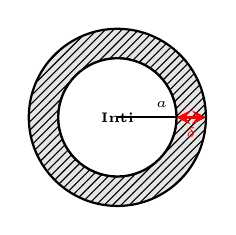
\begin{tikzpicture}[scale=0.75]
    \draw[thick, fill=gray!20] (0,0) circle (1.5);
    \draw[thick, fill=white] (0,0) circle (1.0);
    \pattern[pattern=north east lines] (0,0) circle (1.5);
    \fill[white] (0,0) circle (1.0);
    \draw[thick] (0,0) circle (1.0);
    \draw[->, >=stealth, thick] (0,0) -- (1.5,0) node[midway, above, font=\tiny] {$a$};
    \node at (0,0) [font=\tiny\bfseries] {Inti};
    \draw[<->, >=stealth, red, very thick] (1.0,0) -- (1.5,0) node[midway, below, font=\tiny\bfseries] {$\delta$};
  \end{tikzpicture}%
  }%
\end{minipage}\par

\vfill

% Kotak Formula Rujukan Teknis & Standar Industri
\begin{tcolorbox}[colback=unibblue!3,colframe=unibblue,colbacktitle=unibblue,coltitle=white,boxrule=0.6pt,arc=2pt,left=6pt,right=6pt,top=3pt,bottom=3pt,title=\textbf{\scriptsize FORMULA RUJUKAN TEKNIS \& STANDAR INDUSTRI TERKAIT}]
  \scriptsize
  \begin{itemize}[leftmargin=*, nosep]
  \item Persamaan Diferensial Bessel Orde $n$: $x^2 \frac{d^2 y}{dx^2} + x \frac{dy}{dx} + (x^2 - n^2) y = 0$
  \item Solusi Umum Bessel: $y(x) = C_1 J_n(x) + C_2 Y_n(x)$ ($Y_n(x) \to -\infty$ saat $x \to 0$)
  \item Kedalaman Penetrasi Efek Kulit (*Skin Depth*): $\delta = \sqrt{\frac{2}{\omega \mu \sigma}} = \frac{1}{\sqrt{\pi f \mu \sigma}}$
  \item Standar \textbf{IEC 61089}: Rasio Resistansi AC/DC Konduktor Pejal: $\frac{R_{\text{ac}}}{R_{\text{dc}}} \approx \frac{a}{2\delta}$ untuk $a \gg \delta$
\end{itemize}
\end{tcolorbox}

\newpage
% ==================== HALAMAN 2 ====================

\noindent{\textbf{\color{unibblue}\large BAGIAN II: ANALISIS SISTEM, EVALUASI STANDAR, \& KOMPUTASI JULIA}}\par
\vspace{1mm}

% Soal C4
\noindent\textbf{4. (C4 - Menganalisis \textbar\ Bobot: 20 Poin)}\par\vspace{0.8mm}
{\footnotesize Analisis Rasio Kenaikan Resistansi AC Sesuai Standar \textbf{IEC 61089}: Akibat efek kulit, arus terkonsentrasi di dekat permukaan luar kawat. (a) Turunkan aproksimasi kenaikan resistansi $R_{\text{ac}}/R_{\text{dc}} \approx \frac{a}{2\delta}$ untuk $a \gg \delta$; (b) Analisis mengapa konduktor transmisi daya arus bolak-balik tegangan ekstra tinggi tidak menggunakan konduktor tembaga pejal berpenampang besar melainkan konduktor berkas berpilin (*bundled stranded conductor*).}\par

\vspace{3.5mm}

% Soal C5
\noindent\textbf{5. (C5 - Mengevaluasi \textbar\ Bobot: 20 Poin)}\par\vspace{0.8mm}
{\footnotesize Evaluasi Desain Konduktor ACSR (*Aluminium Conductor Steel Reinforced*): Kawat ACSR menempatkan inti baja di lapisan terdalam dan untaian aluminium di lapisan terluar. Evaluasi keunggulan desain struktur ini secara terintegrasi dari sudut pandang elektromagnetika (rapat arus Bessel Kelvin) dan kekuatan mekanis bentangan antar-menara transmisi.}\par

\vspace{3.5mm}

% Soal C6
\noindent\textbf{6. (C6 - Merancang \& Komputasi Julia \textbar\ Bobot: 15 Poin)}\par\vspace{0.8mm}
{\footnotesize Rancang skrip program ilmiah berbasis \textbf{Julia} menggunakan paket \texttt{SpecialFunctions.jl} untuk menghitung nilai fungsi Bessel $J_0(x)$ dan $J_1(x)$. Program harus memplot kurva distribusi rapat arus ternormalisasi $|J_z(r)/J_0|$ dari pusat kawat ($r = 0$) hingga tepi permukaan ($r = a$) pada tiga variasi frekuensi ($50\text{ Hz}, 500\text{ Hz}$, dan $50\text{ kHz}$).}\par

\vfill

% Tabel Rekapitulasi Skor OBE & Lembar Catatan Umpan Balik Dosen
\noindent\begin{minipage}[b]{0.62\textwidth}%
  \centering
  \scriptsize
  \begin{tabular}{|c|c|c|c|c|c|c|}
    \hline
    \rowcolor{unibblue}
    \textbf{\color{white}C1} & \textbf{\color{white}C2} & \textbf{\color{white}C3} & \textbf{\color{white}C4} & \textbf{\color{white}C5} & \textbf{\color{white}C6} & \textbf{\color{white}Total} \\
    \rowcolor{unibblue!10}
    10 Pts & 15 Pts & 20 Pts & 20 Pts & 20 Pts & 15 Pts & 100 Pts \\
    \hline
    & & & & & & \\[3mm]
    \hline
  \end{tabular}%
\end{minipage}%
\hfill%
\begin{minipage}[b]{0.35\textwidth}%
  \centering
  \scriptsize
  \textbf{Verifikasi Dosen / Asisten:}\\[6mm]
  (\dotfill)\\[1mm]
  \tiny Tanggal: \dotfill
\end{minipage}\par

\vspace{2mm}
\begin{tcolorbox}[colback=white,colframe=unibblue!40!black,colbacktitle=unibblue!10,coltitle=unibblue,boxrule=0.5pt,arc=2pt,left=5pt,right=5pt,top=3pt,bottom=3pt,title=\textbf{\tiny Catatan Evaluasi \& Umpan Balik Dosen Pengampu}]
  \tiny
  \textbf{Rubrik Pemeriksaan Pengerjaan Tugas Mandiri:}\par\vspace{0.8mm}
  $\square$ Penurunan matematis langkah-demi-langkah runtut (C1--C4) \hfill $\square$ Validasi analitis \& standar industri IEEE/IEC/SPLN akurat (C5)\\[0.8mm]
  $\square$ Skrip program Julia mandiri \& grafik visualisasi terlampir (C6) \hfill $\square$ Kerapian format laporan \& ketepatan waktu pengumpulan\\[2.0mm]
  \textbf{Catatan / Koreksi Khusus Dosen:}\\[1.6cm]
\end{tcolorbox}

\end{document}
